\documentclass[10pt,final,conference,letterpaper]{IEEEtran}

\usepackage[utf8]{inputenc}
\usepackage[bookmarks=false]{hyperref} % bookmarks=false required by IEEE upload
\usepackage{flushend} % to equalize length of 2 last cols
\usepackage{xcolor,color,colortbl,graphicx,tabularx}
\usepackage{amssymb, pifont}
\newcommand{\xmark}{\ding{55}}
\usepackage{etoolbox}
\usepackage[para]{threeparttable}
\usepackage{pgfplots}
\usepackage{multirow}
\usepackage{xspace}
\usepackage{cite}
\usepackage[acronym]{glossaries}
\usepackage{booktabs}
\usepackage{todonotes}
\presetkeys%
{todonotes}%
{inline,}{}
\usepackage{comment}

\usepackage{nicefrac}
\usepackage{xfrac}
\usepackage{subfloat}
\usepackage{subcaption}

\usepackage{tikz}
\usetikzlibrary{shapes,arrows,shadows}
\usepackage{amsmath,bm,times}
\usepackage{environ}
\usepackage{tumcolor}
\usepackage{textgreek}

\usepackage[group-minimum-digits=3,group-separator={,}]{siunitx}

\makeatletter
\newsavebox{\measure@tikzpicture}
\NewEnviron{scaletikzpicturetowidth}[1]{%
	\def\tikz@width{#1}%
	\def\tikzscale{1}\begin{lrbox}{\measure@tikzpicture}%
		\BODY
	\end{lrbox}%
	\pgfmathparse{#1/\wd\measure@tikzpicture}%
	\edef\tikzscale{\pgfmathresult}%
	\BODY
}

\newcommand{\apnslong}{Apple Push Notification service\xspace}
\newcommand{\apns}{APNs\xspace}
\newcommand{\pns}{PNS\xspace}
\newcommand{\pnses}{PNSes\xspace}
\newcommand{\man}{metropolitan area network\xspace}
\newcommand{\mans}{metropolitan area network\xspace}
\newcommand{\itunes}{iTunes\xspace}

\newcommand{\packet}[3]{
	\draw[-latex,line width=0.7pt] (#1) to node[above,sloped]{\normalsize{{#3}}} (#2);}

\newcommand{\dpacket}[3]{
	\draw[latex-latex,line width=0.7pt] (#1) to node[above,sloped]{\normalsize{{#3}}} (#2);}

\hyphenation{para-digms}
\hyphenation{para-digm}
\hyphenation{meas-ure-ment}
\hyphenation{meas-ure-ment-ba-sed}
\hyphenation{a-ca-de-mi-a}
\hyphenation{GeoNames}

\urlstyle{same}

\title{Push Away Your Privacy: Precise User Tracking Based on TLS Client Certificate Authentication}


\author{\IEEEauthorblockN{Matthias Wachs, Quirin Scheitle, Georg Carle}
	Chair of Network Architectures and Services\\
	\IEEEauthorblockA{Technical University of Munich (TUM)\\
	Email: \{wachs,scheitle,carle\}@net.in.tum.de}
}

% TMA page limit: 8 pages in IEEE 2-column style, plus an additional page for references.
\begin{document}

\maketitle              % typeset the title of the contribution
% !TEX root = ../tls-cca-privacy.tex
\begin{abstract}%
The design and implementation of cryptographic systems offer many subtle pitfalls.
One such pitfall is that cryptography may create unique identifiers potentially usable to repeatedly and precisely re-identify and hence track users.
This work investigates TLS Client Certificate Authentication (CCA), which currently transmits certificates in plain text.
We demonstrate CCA's impact on client traceability using Apple's {\apnslong} (APNs) as an example. {\apns} is used by all Apple products, employs plain-text CCA, and aims to be constantly connected to its backend.
Its novel combination of large device count, constant connections, device proximity to users and unique client certificates provides for precise client traceability.
We show that passive eavesdropping allows to precisely re-identify and track users and that only ten interception points are required to track more than 80 percent of {\apns} users due to global routing characteristics.
We conduct our work under strong ethical guidelines, responsibly disclose our findings, and can confirm a working patch by Apple for the highlighted issue.
We aim for this work to provide the necessary factual and quantified evidence about negative implications of plain-text CCA to boost deployment of encrypted CCA as in TLS 1.3.
\end{abstract}%
% !TEX root = ../tls-cca-privacy.tex
\section{Introduction}\label{sec:intro}
Encryption offers a wide range of security benefits and is praised by companies to offer security to their customers~\cite{2016cook}. 
A side-effect of cryptography can be the creation of unique cryptographic identifiers, which can, for example, be observed in TLS authentication using X.509 certificates.
TLS, including its current version 1.2, sends server and client certificates in plain text before establishing an encrypted channel.
Client certificates may contain sensitive user information such as users' real names.
Even if these certificates do not leak personal information directly, the client certificates, typically valid and used for several years, establish unique markers for precise identification across repeated observations.
In this work, we demonstrate the privacy impact of \emph{Client Certificate Authentication (CCA)} used by Apple's \emph{{\apnslong} ({\apns})}.
With over 1 billion active Apple devices in the world~\cite{apple1bn}, of which many are used by politicians, journalists, or other high-profile groups, this service is relevant in both size and the demographics of its user base.
As {\apns} tries to hold an active connection to its backend servers at
all times, tracking users through this connection is promising.

Unique information contained in certificates enable both local and
global adversaries with access to network traffic to uniquely identify users,
track them over time, and create profiles of their behavior and usage patterns.
While existing methods based on traffic correlation or traffic markers only allow
to identify users with a certain \textit{probability}, client certificates allow \textit{precise}
identification of users or user devices.

In this work, we demonstrate the exploitability of unique CCA identifiers leaked current TLS as used by {\apns}.
We do so by 
(i) using passive measurements to verify precise re-identification and traceability of certificates in a large \man, and 
(ii) using active measurements to show that {\apns} logins are globally routed through few central networks, potentially susceptible to a powerful attacker. 

Having established both feasibility and impact of this privacy leakage, we follow a responsible disclosure process and report our findings to Apple's Product Security Team. 
In a very positive exchange, Apple confirmed our findings and its privacy implications.
Apple has been diligently working on a patch to resolve this issue, which is included as CVE-2017-2383 in the iOS 10.2.1 and macOS 10.12.3 security updates released on January 23, 2017~\cite{ios1021}.

We see the main contributions of our work in:
\begin{itemize}
	\item Measuring evidence on the privacy and traceability impacts of clear-text CCA
	\item Proving that a powerful global adversary may easily and passively leverage CCA to track users globally
	\item Following through the disclosure and patch process to protect the large {\apns} user base from this vulnerability
\end{itemize}
We aim for this example to be taken seriously by other applications using TLS CCA, and hope to boost the deployment of encrypted CCA through several strategies, including TLS 1.3, discussed in this paper. 

We structure our work as follows: 
We give background in Section~\ref{sec:background} and discuss related work in Section~\ref{sec:related}.
We define the attacker model in Section~\ref{sec:attacker}, followed by passive TLS CCA observations in Section~\ref{sec:verloc}, and a dissection of {\apns}'s global routing in Section~\ref{sec:routing}. 
We discuss our findings and their disclosure in Section~\ref{sec:disclosure}, before concluding our work in Section~\ref{sec:summary}.

% !TEX root = ../tls-cca-privacy.tex
\section{Background}\label{sec:background}
This section gives background on TLS and CCA, push notification services in general, and {\apns} and its employment of TLS CCA in particular.
%
\subsection{TLS \& Certificate-Based Authentication}\label{sec:tls}
%
Transport Layer Security (TLS)---often mistakenly still called SSL---is the de facto standard to establish secure communication between systems on today's Internet.
The most noticeable benefit of TLS is that it allows to provide secure communications without modifying or impacting higher-layer protocols.
The latest version 1.2 of TLS is defined in RFC\,5246. %
The first draft of TLS\,1.3~\cite{ietf-tls-rfc5246-bis-16} was published in 2014 but standardization is still work in progress.
TLS provides mechanisms to authenticate both the destination (server) and the initiator (client) of a connection.

The following explanation focuses on authentication and certificate-related aspects of the TLS 1.2 handshake. 
When a client establishes a TLS connection, it first sends a \textit{ClientHello} message, containing the cryptographic ciphers
supported by the client and other information. 
The server responds with a \textit{ServerHello} followed by a \textit{Certificate} message containing one or more certificates to authenticate the server. 
In addition, the server can request a certificate from the client by sending a \textit{CertificateRequest} message. 
This message may include a list of desired Certificate Authorities (CAs) supported for validation. 
The client responds with a \textit{Certificate} message containing the client's certificate chain. 
Only after this unencrypted mutual authentication, both partners establish the desired secure channel. 
A TLS 1.2 mutual authentication is depicted in Figure~\ref{fig:tls12tikz}.

% !TEX root = ../tls-cca-privacy.tex
\begin{figure}
\begin{subfigure}{0.48\textwidth}
\resizebox{\textwidth}{!}{
		\begin{tikzpicture}
\node at ([yshift=.1cm] 0,0) [anchor=south,minimum width=1cm] {Client};
\node at ([yshift=.1cm] 7,0) [anchor=south,minimum width=1cm] {Server};

\draw[-latex,line width=1.4pt] (0,0) to (0,-4.5);
\draw[-latex,line width=1.4pt] (7,0) to (7,-4.5);

% Client Hello is first TLS message , see https://tools.ietf.org/html/rfc5246#section-7.3:
\packet{0,-.5}{7,-.7}{\textcolor{black}{ClientHello}};
\packet{7,-1.7}{0,-1.9}{
		\begin{tabular}{c}
		\textcolor{black}{ServerHello, Certificate,} \\
		\textcolor{black}{\ldots, CertificateRequest, \ldots}
		\end{tabular}
	}

\packet{0,-2.4}{7,-2.6}{\textcolor{black}{Certificate,\ldots , }\textcolor{TUMBlue}{\underline{\textbf{{Finished}}}}};
\packet{7,-3.1}{0,-3.3}{\textcolor{TUMBlue}{\underline{\textbf{{Finished}}}}};
\dpacket{7,-3.9}{0,-3.9}{\textcolor{TUMBlue}{\underline{\textbf{{[Application Data]}}}}};

		\end{tikzpicture}
	} % end resizebox

\caption{TLS 1.2 Handshake}
\label{fig:tls12tikz}
\end{subfigure}
\quad
\begin{subfigure}{0.48\textwidth}
\resizebox{\textwidth}{!}{
	\begin{tikzpicture}

	\node at ([yshift=.1cm] 0,0) [anchor=south,minimum width=1cm] {Client};
	\node at ([yshift=.1cm] 7,0) [anchor=south,minimum width=1cm] {Server};

	\draw[-latex,line width=1.4pt] (0,0) to (0,-4.5);
	\draw[-latex,line width=1.4pt] (7,0)  to (7,-4.5);
	% Details: https://tlswg.github.io/tls13-spec/#rfc.section.2
	\packet{0,-0.5}{7,-0.7}{\textcolor{black}{ClientHello}}
	\packet{7,-2.2}{0,-2.4}{
		\begin{tabular}{c}

		\textcolor{black}{ServerHello},\\ 
		\textcolor{TUMBlue}{\underline{\textbf{\ldots, Certificate, CertificateRequest,}}} \\ 
		\textcolor{TUMBlue}{\underline{\textbf{\ldots, Finished, [Application\,Data]}}} 
		\end{tabular}
	};

	\packet{0,-3.1}{7,-3.3}{\textcolor{TUMBlue}{\underline{\textbf{{Certificate, \ldots, Finished, [Application Data]}}}}} ;
	\dpacket{7,-3.8}{0,-3.8}{\textcolor{TUMBlue}{\underline{\textbf{{[Application Data]}}}}};

	\end{tikzpicture}
}
\caption{TLS 1.3 Handshake}
\label{fig:tls13tikz}
\end{subfigure}\\
\caption{Handshakes in TLS\,1.2 and TLS\,1.3 (draft), highlighting unencrypted and \textcolor{TUMBlue}{\underline{\textbf{encrypted}}} data. Both client and server certificates are encrypted in TLS\,1.3.}
\vspace{-1em}
\end{figure}


For authentication, TLS relies on X.509v3 certificates~(cf. RFC\,5280),
asserting that a cryptographic public key belongs to the certificate's \emph{subject},
making certificates identifiable and attributable to users or devices.
Certificate validation is performed by the system receiving the certificate. 
Validation is performed according to the system's requirements, i.e., the systems do not have to use publicly verifiable certificates issued by well-known certificate authorities but can instead rely on private CA infrastructures.

The current draft for TLS 1.3~\cite{ietf-tls-rfc5246-bis-16} proposes a
different handshake protocol with the specific security goal to protect the
endpoints' identities. First of all, a shared secret is established between
client and server to protect against passive attackers. The client first sends a
\textit{ClientHello} message containing an (EC)DHE key share. The server
responds with a \textit{ServerHello} message containing its key share used to
compute the shared secret. After such a shared secret is established and
communication is encrypted, the server provides the client with its certificate
in the \textit{Certificate} message. Only after sending its certificate, it can
request a client certificate sending a \textit{CertificateRequest} message.
This approach protects both the server and client certificate from observation. 
The proposed handshake for TLS 1.3 is depicted in Figure~\ref{fig:tls13tikz}.
It is important to note that TLS 1.3 can still leak sensitive information since the \textit{ClientHello} (containing the TLS extensions) is still unencrypted. 
These TLS extensions can, for example, leak the target hostname through the \textit{Server Name Indication (SNI)} \textit{ClientHello} extension.


%%%%%%%%%%%%%%%%%%%%%%%%%%%%%%%%%%%%%%%%%

\subsection{Use Cases for Client Certificate Authentication}

TLS in combination with CCA is used in a large
variety of settings, especially when mutual authentication of communication
partners is essential. 
Where passwords are considered insufficient, CCA can provide a level of multi-factor authentication, as recommended by OWASP~\cite{OwaspCCA}.

On network level, CCA can be used with network access control and virtual private
network authentication. One prominent example is enterprise (wireless) network
authentication using 802.1x in combination with the \emph{Extensible Authentication
Protocol (EAP)} (cf. RFC\,5247). EAP is an extensible authentication framework
and supports certificate-based mutual authentication with EAP-TLS (cf. RFC\,5216).
TLS CCA is also used with OpenVPN~\cite{OpenVpn}, one of the most widely used solutions
to create virtual private networks (VPN). OpenVPN uses a custom security
protocol based on shared keys or TLS. In TLS mode, OpenVPN employs X.509
certificates for mutual authentication.

With HTTPS, TLS can be used to authenticate both the web site and the user.
Popular web servers such as Apache, NGINX, and IIS support authentication using CCA.
Websites do not widely use CCA as it is complex for users to install and maintain certificates across multiple devices and browsers.

{\noindent}TLS and CCA are also employed for higher-layer applications such as MQTT (cf. ISO/IEC PRF 20922), a lightweight messaging protocol designed for the ``Internet of Things''. 
MQTT can use TLS and CCA for client authentication, but provides no means to authenticate the server.

\subsection{Push Notification Services}

\textit{Push Notification Services ({\pnses})} are an essential functionality of modern
service ecosystems. 
{\pnses} provide a resource efficient approach for service backends to notify (mobile) devices and applications about
events. 
{\pnses} originate from mobile platforms where resources like energy and network access are limited.
%
All modern mobile platforms are equipped with {\pnses}, often tightly integrated with the operating system: 
Apple's {\apns} on iOS, Firebase Cloud Messaging (FCM) on Google's Android, and Windows Notification Service (WNS) on Windows Phone are prominent examples. 
{\pnses} became the most prominent way to notify applications about service events. 
{\pnses} are also integrated with desktop operating systems and even web browsers (e.g., Google FCM in Chrome) to efficiently notify applications about service events. 
This makes {\pnses} an omnipresent, inevitable link between applications, devices, and service and infrastructure backends. 
Figure~\ref{fig:pstikz} displays this basic concept of {\pnses}.
% !TEX root = ../tls-cca-privacy.tex
%%%%%%%%%%%%%%%%%%%%%%%%%%%%%%%%%%%%%%%%%
\begin{figure}
\begin{scaletikzpicturetowidth}{1\linewidth}
	\begin{tikzpicture}[scale=\tikzscale]
	\pgfdeclarelayer{bg}    % declare background layer
	\pgfsetlayers{bg,main}
	% Push Server
	\draw [fill=white] (4,2) rectangle (6,0) node [pos=0.5,yshift=5] {Push} node [pos=0.5,yshift=-5] {Server};

	% Phone
	\draw [rounded corners] (9.5,0) rectangle (11.2,2) ;
	\draw[rounded corners] (9.6,.4) rectangle (11.1,1.9);
	\draw (10.4,.2)--(10.4,.2);
	\draw[->,dashed](6,1) -- (9.5,1);

	% Servers
	\draw [fill=white] (0,-.5) rectangle (2.25,-1.5) node [pos=0.5] {Server C} ;
		\draw[thick](2.25,-1) -- (4,1);
	\draw [fill=white] (0,.5) rectangle (2.25,1.5) node [pos=0.5] {Server B} ;
		\draw[thick](2.25,1) -- (4,1);
	\draw [fill=white] (0,2.5) rectangle (2.25,3.5) node [pos=0.5] {Server A} ;
		\draw[thick](2.25,3) -- (4,1);

	% Apps
	\draw [fill=white, rounded corners=2mm] (13,-.5) rectangle (15,-1.5) node [pos=0.5] { App C} ;
			\draw[thick](11.2,1) -- (13,-1);
	\draw [fill=white, rounded corners=2mm] (13,.5) rectangle (15,1.5) node [pos=0.5] { App B} ;
			\draw[thick](11.2,1) -- (13,1);
	\draw [fill=white, rounded corners=2mm] (13,2.5) rectangle (15,3.5) node [pos=0.5] { App A} ;
			\draw[thick](11.2,1) -- (13,3);

	\end{tikzpicture}
\end{scaletikzpicturetowidth}
%
\caption{Push Service Architecture: Messages brokered to Apps through the Push Notification Service.}
\label{fig:pstikz}
\end{figure}


When establishing a connection to the {\pns}, both the device and the
third party provider have to authenticate to the service. While for third party
provider, authentication approaches like OAuth are used, device authentication is
not documented for most services due to their proprietary architecture and
tight integration with the operating system. Only Apple documents the use
of TLS and CCA with its security guide~\cite{IosSecurityGuide} and {\apns} documentation~\cite{2016appleapns}.
We investigate communication for Google's FCM and Microsoft's WNS, but do not
find plain-text client certificates. Google's FCM uses TLS 1.2 and TCP ports 5228 through
5230 to connect to its backend. In our analysis for FCM, no
unencrypted client certificates were transmitted with the handshake. The same applies
to Microsoft's WNS, which uses TCP port 443 and TLS 1.2. 

\subsection{{\apnslong} ({\apns})}
\label{sec:apns}
% CONSISTENCY: The current Mac operating system is macOS, originally named "Mac OS X" until 2012 and then "OS X" until 2016.[3] 
%
Within Apple's ecosystem, \apns is a key service for the communication between Apple's service backend and user devices and applications. 
{\apns} was added to mobile devices with iOS 3.0 in 2009, and extended macOS platforms with the release of Mac OS X 10.7 in 2011. 
{\apns} and CCA is also used with \itunes on Windows 7 and later. 
Support for website notifications in Apple's Safari browser was added with the release of Mac OS X 10.9 in 2013.

On its initial activation, each Apple device is provided with a private cryptographic key and a X.509
certificate, stored in the device keychain.
With \itunes, the certificate is created when logging in with
an Apple ID and is stored in Window's certificate store. Mutual authentication
is performed when the device connects to {\apns}: Using TLS 1.2 with CCA as
described in Section~\ref{sec:tls}, first the server's certificate is validated
by the device. Next, the device sends its client certificate, which is validated
by {\apns} to establish a mutually trusted connection~\cite{2016appleapns}.

For \textit{device-to-push-service} communication, {\apns} uses two different TCP
ports~\cite{2016appleapnstrouble}: By default the device tries to connect to an
{\apns} server on TCP port 5223. If TCP port 5223 is not reachable (e.g., due to
port filtering), {\apns} connects to TCP port 443 on WLAN only.
% 
When connected to both cellular and WLAN or wired networks, {\apns} prefers cellular data
links over WLAN or wired connections~\cite{2016appleapnstrouble}. 
We assume this reduces reconnects and provides a stable link for mobile users.

For its backend, {\apns} employs a load balancing architecture, where
devices connect to one of 50 {\apns} DNS records named
\textit{{[1-50]-courier.push.apple.com}}~\cite{2016appleapnstrouble}. 
These names are served by Akamai's DNS service and mapped to
\textit{{[1-50]\-.courier\--push\--apple\-.com\-.akadns\-.net}}
using CNAME records. 
These resolve to a geographically close name, for example, 
\textit{{pop\--eur\--central\--courier\-.push\--apple\-.com\-.akadns\-.net}}
when resolved from Munich. 
These names resolve to a variety of IP addresses in Apple's 17.0.0.0/24 address range.
%

% !TEX root = ../tls-cca-privacy.tex
\section{Related Work}
\label{sec:related}

To the best of our knowledge, only limited work on the privacy
implications of digital certificates with a particular focus on 
certificate-based client authentication exists. In particular, no assessment of
real world implications of CCA exists.

Parsovs~\cite{parsovs14clientauth} gives an extensive overview of operational problems
related to TLS CCA. He rather addresses implementation details than general privacy implications, but also highlights that
client certificates should not be transmitted in clear text.
He mentions TLS modifications proposed for standardization that ensure encrypted transport of client certificates,   
but notes that a modification of the TLS standard would take years to be adopted.
He explores how renegotiation, as a possible workaround for an encrypted transmission of client certificates, has a negative impact on performance. 
%
Aura and Ellison~\cite{Aura00privacyand} analyze privacy implications of
certificates and certificate systems in detail, and highlight identity leakage and
unique keys as main issues with certificates. The authors describe several
anonymity techniques such as key-oriented access control and certificate reduction
as solutions to these problems, and how the SDSI PKI, a distributed PKI proposed by 
Rivest and Lampson in~\cite{RivestSDSI}, leverages
these techniques. For X.509, these approaches were never adopted.

Chung et al.~\cite{chung2016measuring} recently tracked over 5M devices for more than one year by actively scanning for invalid X.509 certificates.
In contrast to our study, active scans can not discover TLS client certificates.
Also, they rather find servers, such as home routers or storage devices, than mobile client devices. 

In an Internet-Draft~\cite{TLSencRay}, Ray highlights the issues of
TLS's unencrypted handshake and its implications with the goal to extend TLS
with an encrypted handshake. Ray proposes to establish a secure connection first 
by exchanging (EC)DH parameters and only then to transmit 
certificates using a second \emph{ClientHello} and \emph{ServerHello} command. 
The draft expired in May 2012 without being adopted.

Langley authored an Internet-Draft~\cite{TLSencLangley} aiming to extend the TLS handshake
with an encrypted certificate. He proposes to first establish an encrypted
connection using the \emph{ChangeCipherSpec} command and only exchange certificates after this step. This approach introduces incompatibilities into the TLS protocol. The draft was not adopted and expired in April 2012. 

In literature, unique identifiers and certificate based authentication in particular are long known to create issues for user privacy.
Nonetheless, neither were these issues addressed in the TLS standard up to TLS 1.2,  
nor was the current TLS 1.2 standard modified, nor was one of the suggested approaches adopted to counteract this issue.
%
While TLS 1.3 addresses this problem, full adoption of TLS 1.3 by services and clients will take a long time with user privacy being at risk. 
To the best of our knowledge, no scientific work tried to analyze or quantify the impacts of CCA on user privacy and the possibility for user tracking, especially in combination with always-connected mobile personal devices. 

Besides cryptographic traceability, unique device identifiers have attracted privacy concerns and mitigation actions: 
Mobile devices used to be well traceable through WLAN MAC addresses. 
This was mitigated years ago by Apple and other vendors by
offering random MAC addresses to unknown networks~\cite{vanhoef2016mac}, 
though not always effectively, as recent work indicates~\cite{martin2017study}.
With IPv6, stateless autoconfiguration calculates an IPv6 address based on the 
network interface's MAC address, with the threat of global traceability of devices.
To protect against such tracking, IPv6 privacy extensions~(cf. RFC~4941) randomly select IPv6 addresses.

There exists a large body of work on tracking users through DNS~\cite{krishnan2010dns}, Mobile Apps~\cite{recon16}, Browser Fingerprinting~\cite{acar2014web} and many other means.
We consider these approaches different from ours in that they are either (i) stochastic, i.e., not leveraging cryptographically unique fingerprints, or (ii) active, i.e., requiring attacker capabilities beyond listening.

% !TEX root = ../tls-cca-privacy.tex
\section{Attacker and Threat Model}\label{sec:attacker}
We define three types of attackers with different motivations and capabilities. 
These attackers are specific points in a possible spectrum of attackers.

Attacker (a) is a powerful entity interested in precisely tracking and identifying users globally.
It is modeled after a nation state or a member of the intelligence community.
This attacker can read network traffic of one or several large Internet backbone networks and/or Internet Exchange Points (IXPs).
In addition, this attacker can typically coerce network operators to provide extended information about users, for example, by mapping IP addresses to network locations.

Attacker (b) is a local or regional entity with access to a single large network.
It could typically be an individual organization or company, with an interest to track roaming and usage patterns of users over different parts of the network.

Attacker (c), the operator of a small network, could also enhance
its tracking capabilities by the use of TLS client certificates, but can already
precisely track typical counts of $<$$10$ users through device names or MAC
addresses. We hence exclude attacker (c) from further analysis.

Currently, attackers (a) or (b) typically will resort to stochastic or opportunistic ``markers'' to identify people.
For example, in the NSA's QuantumInsert program, some markers (``realms'') used are Facebook, HotMail, or YouTube cookies as well as public static IPv4 addresses~\cite[p. 5]{effqi}.
In contrast to the markers mentioned above, we highlight that client certificates used by TLS CCA are cryptographically unique, used by different services, rarely change over time, are wide-spread on billions of devices, and are frequently transmitted, especially when used with mobile devices and always connected services, such as mobile push notification services.

We highlight that attackers (b) and (c) typically also have other possibilities of tracking users within their own networks, based on, for example, MAC addresses or, for cellular operators, IMEI identifiers.
We also emphasize that tracking users based on TLS Client Certificates requires only passive network access, enabling attacks to be conducted (i) in a lightweight manner, and (ii) retrospectively on stored network samples.
% !TEX root = ../tls-cca-privacy.tex
\section{Verification of \\Metropolitan Area Network Traceability}\label{sec:verloc}
\label{sec:results}
This section emulates attacker (b) as defined in Section~\ref{sec:attacker}, which has interception capabilities in a \man.
We verify that this attacker can effectively track users through passive measurements.

\subsection{Experimental Setup and Methodology}\label{sec:exp}
To give a detailed analysis and evaluation of {\apns} communication patterns and
to be able to analyze the impact of {\apns}'s use of CCA on user privacy in the \man attacker scenario, we conduct an
extensive analysis of {\apns} communication. This scenario does not include
mobile cellular connections, but only WLAN and wired connections.


We monitor {\apns} communication at the Internet uplink of the Munich Scientific Network (MWN), a \man connecting about 100,000 users to the Internet.
We consider the MWN an insightful environment as it provides properties of scientific (connecting several large universities), corporate (employees at various organizations), and residential (student residence halls) networks.

Using \textit{tcpdump}, we capture {\apns} TLS handshake packets containing certificates over the course of 17 days.
We employ a \textit{pcap} filter for TCP traffic with destination ports 443, 5223, 2195, and 2196 used by {\apns} as described in Section~\ref{sec:apns}.
The filter also limits capturing to TLS handshake protocol
messages (\textit{Record Layer ContentType} = \textit{handshake}) containing certificate
information (\textit{Handshake Type} = \textit{Certificate}).

We capture data as \textit{pcap} files and use a python processing tool
leveraging \textit{scapy}~\cite{scapy} extended with
\textit{scapy-ssl\_tls}~\cite{scapytls} to extract certificate information.
Using this tool, we extract the following information from the \textit{pcap} files:

\begin{itemize}
	\item \textbf{Connections: }%
	timestamp, source IP address, source port, destination IP, destination port, certificates found
	\item \textbf{Certificates: }%
	X.509 version, serial number, subject, issuer, public key modulus, public key size, start and end of validity, fingerprint, extensions contained
	\item \textbf{Certificate extensions: }%
	name/OID and values
\end{itemize}

{\noindent}While processing, we perform DNS reverse resolution for source and destination IP addresses to obtain DNS hostnames.

\subsection{Ethical Considerations}\label{sec:ethical}

We follow an internal multi-party approval process before any measurement
activities are carried out. This approval process incorporates the proposal of
Partridge and Allman~\cite{partridge2016ethical} to assess whether the
collection of data can harm individuals and whether the collected data
reveals private information.

The focus of this work is solely to create profiles of devices. We do not
attempt create a link between devices (i.e., the certificates found) and the
respective owner's identity, except five members of our research group giving informed consent to case studies.
Information contained in the certificates does not provide a possibility to directly link it with a user. 
We neither try to link certificates to users based on identifiers such as IP addresses, nor try to uncover their geographical location.

The measurements conducted for this work were performed on an isolated measurement infrastructure not accessible from the Internet. 
Data obtained in our measurements must remain on this infrastructure. 
%
The methodology for this experiment was thoroughly documented before the measurement was conducted.
The experiment's methodology fully complies with the strict code of conduct required by our internal ethical review processes, and we obtained approval for our measurements in this process. 
We hence conclude it is ethical to conduct the experiment, but will, in contrast to our usual policy, not share raw data from this work with the public.


\subsection{Properties of {\apns} Certificates}
Our experiments show that \apns, relying on standard TLS 1.2, employs
standard X.509v3 certificates for mutual authentication between devices and
{\apns} servers. {\apns} devices use 1024 bit RSA keys and are provided with
certificates issued by an \textit{Apple iPhone Device CA} certificate authority
using the common name \texttt{\footnotesize{C=US, O=Apple Inc., OU=Apple iPhone,
CN=Apple iPhone Device CA}}.


Our investigations show that certificates of mobile devices (iPhones, iPads)
running iOS have different properties than certificates of desktop devices
running macOS and \itunes on Windows. This allows us to distinguish between mobile
and desktop devices: certificates for mobile devices have a subject containing a
unique identifier and CA information similar to
\texttt{\footnotesize{CN=7F3F3123\--1234\--4EF8\--5678\--F3CDE236E1EF, C=US,\-
ST\-=CA,\- L=Cupertino, O=Apple Inc., OU=iPhone}}. 
In contrast, certificates for desktop devices only contain the unique identifier:
\texttt{\footnotesize{CN=7F3F3123-1234\--4EF8\--5678\--F3C\-DE\-236\-E1EF}}.
By investigating several devices of consenting users, we verify that the certificate's \emph{``not valid before''} timestamp reflects the precise time of device registration with Apple.
The certificate validity for iOS devices is 3 years, while certificates for desktop devices only have a validity of 1 year.

\subsection{Data Capturing and Basic Statistics}
%
Capturing for 17 days in September 2016, we observe 70,173,492 TLS CCA connections with 57,477 unique client certificates, of which 56,128 (97\%) stem from \apns.
Across all 57,477 client certificates, we find 220 distinct issuer distinguished names (\textit{DNs}). % in those 57,477 client certificates, 
The Top 5 issuer \textit{DNs} are shown in Table~\ref{tab:issuercn}, exhibiting a clear dominance of {\apns} certificates in our data set, 
but also showing other use cases of CCA such as client service authentication and remote device management.

\begin{table}
	\centering
	\caption{Number of observed TLS client certificates for five most frequent Issuer Distinguished Names.}%
	 \resizebox{\columnwidth}{!}{
	\begin{tabular}{ll}
		\toprule
		\#Certs & Issuer Distinguished Name \\
		\midrule
		56128 & /C=US/O=Apple Inc./OU=Apple iPhone/CN=Apple iPhone Device CA \\
		334 & /CN=Layer Client CA/C=US/L=San Francisco/O=Layer, Inc/ST=CA \\
		221 & /CN=AnyDesk Client \\
		76 & /C=KR/ST=Kyunggido/L=Suwon/O=Samsung Electronics (\textit{redacted})\\ 
		52 & /CN=Ricoh Remote Service (\textit{redacted})\\ 
		\bottomrule
	\end{tabular}
	}
	\label{tab:issuercn}
	\vspace{-1em}
\end{table}

The 56,128 {\apns} certificates can further be broken down into 40,313 (72\%) iOS certificates and 15,815 (28\%) desktop certificates.
Of the 70,173,492 TLS CCA connections, we identify 68,231,915 as {\apns} certificates on port 5223 and 1,588,864 as {\apns} certificates on port 443.
The small remainder of 352,713 connections did not use {\apns} certificates.

\subsection{Recurrence of Certificates}
To assess whether the described capture would allow for reliable traceability of users, we first investigate the recurrence of certificates: Only certificates observed more  than once allow for a basic level of user tracking. Figure~\ref{fig:connspercert} displays the number of connections observed per certificate.

\begin{figure}%
	\centering
	\begin{subfigure}{\columnwidth}%{0.48\textwidth}%
		\href{https://github.com/tumi8/cca-privacy/blob/master/analyses/results/1_connections_per_certificate.ipynb}{%
		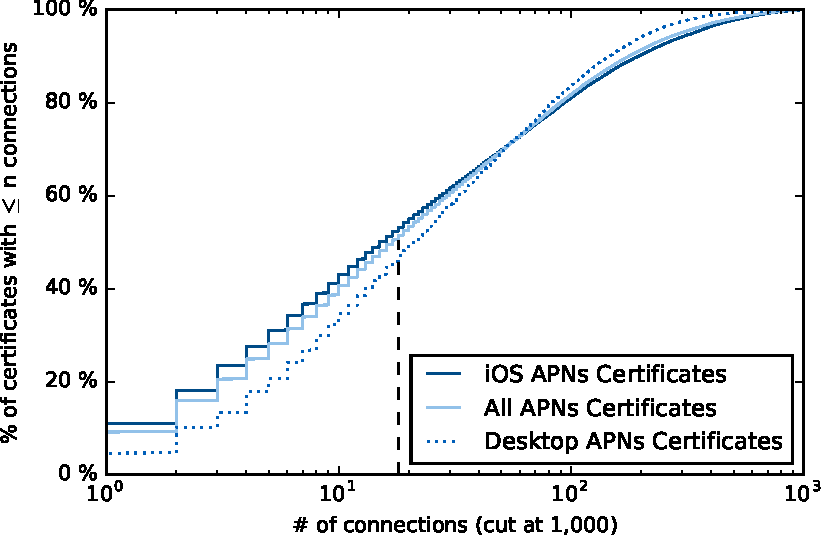
\includegraphics[width=\textwidth]{figures/connspercert-crop.pdf}%
		}
		\caption{$\sim$50\% of certificates observed with more than 17 connections, 9\% of certificates only observed once (5\% desktop, 11\% iOS).}
		\label{fig:connspercert}
	\vspace{3mm} % manually align figure layout
	\end{subfigure}
	\begin{subfigure}{\columnwidth}%{0.48\textwidth}%
		\href{https://github.com/tumi8/cca-privacy/blob/master/analyses/results/1_connections_per_certificate_per_day.ipynb}{%
		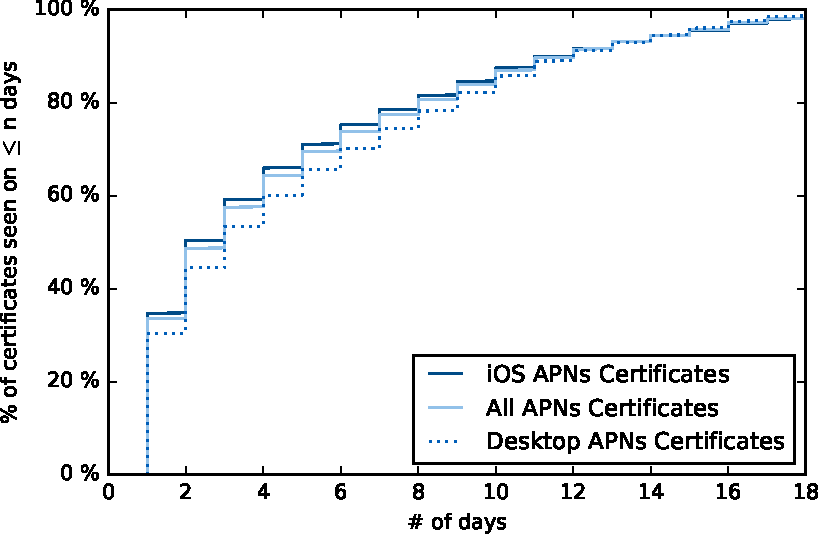
\includegraphics[width=\textwidth]{figures/connspercert_per_day-crop.pdf}%
		}
		\caption{50\% of certificates observed on 3 or more separate days, 34\% only observed on 1 day (30\% desktop, 35\% iOS).}
		\label{fig:connspercert_per_day}
	\end{subfigure}
	\caption{Statistics on certificate recurrence --- \emph{Click on any data-driven figure in this paper to go to its source code}}
	\label{fig:connspercert_big}
	\vspace{-3mm} % avoid ugly linebreak in section V-F
\end{figure}

We display total number as well as a breakdown into iOS and desktop devices. We
find about 50\% of total certificates to have 17 or more connections. The fact
that only $\leq$10\% of certificates are only observed once speaks to
traceability of individual certificates. Please note that 95\% of desktop
certificates were observed more than once, as desktop devices typically can not connect
to {\apns} through cellular service, hence always use our observed WLAN or wired connections to
connect. We find some certificates with dozens of millions of connections, which
we can link to an iOS continuous integration build cluster within the network.
Figure~\ref{fig:connspercert_per_day} displays the number of days that
individual certificates were observed to connect on. About 50\% of certificates
connected on 3 or more days. We consider these regular users of our network,
which are likely well traceable over longer periods.

\subsection{Deductions about User Behavior}
We next set out to explore the level of insight that can be deduced about
individual users and devices.

Figure~\ref{fig:userstudy-1} tracks the {\apns} certificate of one of
the authors' MacBook to ensure applicability of our methodology and
highlight the relevance of our work. Based on the subnet of the source IP address, we can
track whether this user logged in from his desk, through WLAN, or through VPN.
% 
Days off and days with outside meetings can clearly be identified, for example, 
the first Monday, with a remote VPN login followed by desk presence later that day.
Meetings away from desk are visible through WLAN logins, for example, the second
Wednesday and Thursday. 
This exhibits the power of tracking users from \apns certificates at a \man level. 
This information is also accessible to eavesdroppers on the path between this \man and the {\apns} backend. 
The mapping of IP addresses to certain networks and characteristics may seem difficult for outsiders, but is eased by descriptive reverse DNS names deployed in these networks.

\begin{figure}%
	\centering
		\href{https://github.com/tumi8/cca-privacy/blob/master/userstudy/userstudy.ipynb}{%
		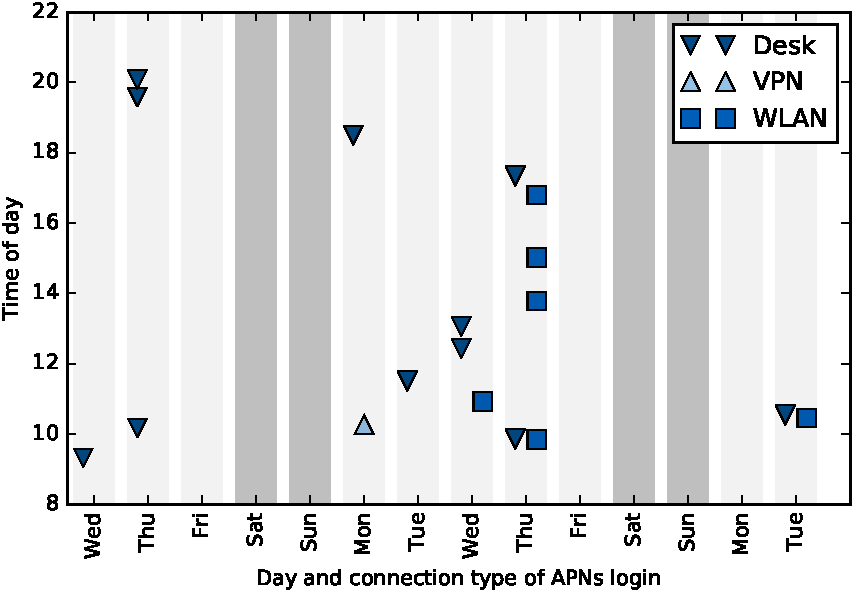
\includegraphics[width=.94\columnwidth]{figures/userstudy-crop.pdf}%
		}
		\caption{User Study: {\apns} logins clearly show work starting times and locations (derived from subnet data).}
		\label{fig:userstudy-1}
		\vspace{-3mm}
\end{figure}
\subsection{Deductions about Devices}

As the certificate's \emph{``not valid before''} timestamp reflects the precise time of device registration with Apple, this can narrow down the device type, as Apple typically stops selling
previous hardware models with the availability of new devices. This means that
the majority of certificates created at a certain point of time will belong to devices from the Apple hardware offerings at that time.

Figure~\ref{fig:certsvalid} depicts the cumulative distribution of the ``\emph{not valid before}'' timestamps in observed {\apns} certificates.
%
\begin{figure}%
	\href{https://github.com/tumi8/cca-privacy/blob/master/analyses/results/2_certificates_valid_from_anon.ipynb}{%
	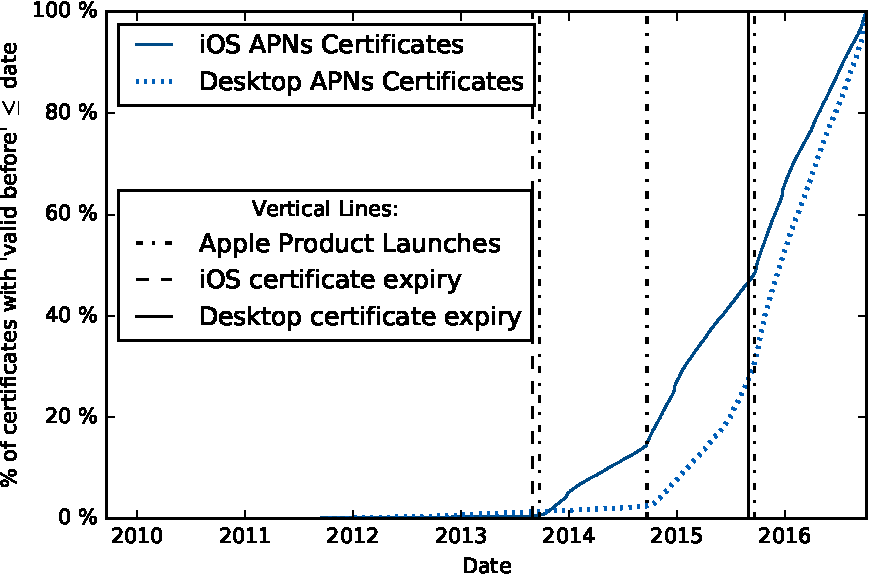
\includegraphics[width=\columnwidth]{figures/certs_valid_from-crop.pdf}%
	}
	\caption{CDF of ``\emph{not valid before}'' timestamps of {\apns} certificates. Highlighted are the influence of Apple's end of September product launches as well as the expiry threshold dates for iOS certificates, which are valid for three years, and desktop certificates, which are valid for one year.}
	\label{fig:certsvalid}
\end{figure}%
Several observations can be taken from this figure:

First, certificates are used beyond their expiry date. As certificates are
valid for 3 years for iOS and 1 year for desktop devices, we can plot the expiration threshold
of certificates in Figure~\ref{fig:certsvalid}.
Certificates issued before these thresholds have exceeded their validity period.

We can see that 28\% of desktop and 1\% of mobile devices use expired certificates.
% source for 28% and 1% numbers:  jupyter notebook analyses/results/2_certificates_valid_from.ipynb
We conclude that {\apns} clients do not systematically renew their certificates and only
re-installations or re-registrations cause certificate renewals over time.
This lack of systematical certificate renewal extends the possible duration a device
can be traced.
Furthermore, Apple's product presentations in end of September typically boost registration of new devices and therefore certificates.

% !TEX root = ../tls-cca-privacy.tex
\section{Global Routing of APNS}\label{sec:routing}
In this chapter we investigate whether a powerful attacker, as described as attacker (a) in Section~\ref{sec:attacker}, can effectively track individual users by eavesdropping on central Autonomous Systems (ASes) or Internet Exchange Points (IXPs).

Based on Apple's documentation~\cite{2016appleapnstrouble} and confirmed by measurement, we establish that (i) {\apns} uses IP addresses from the \textit{17.0.0.0/8} prefix and (ii) devices resolve one of \textit{[1-50]-courier.push.apple.com} to connect to an individual {\apns} server.
We globally resolve those DNS names through RIPE Atlas and find them to redirect, based on resolver location, into several regional Akamai clusters (located in Apple's \textit{17.0.0.0/8} IP range), featuring a total of 69 subnets of size /24.
In the next step, we randomly pick one of the observed IP addresses in each of the 69 /24 subnets, resulting in 69 measurement targets.
We then conduct in-protocol (using TCP/5223) \textit{traceroute} measurements towards each of the 69 targets, selecting 1000 random globally distributed probes for each measurement.
Over all 69 global traceroute measurements, we use a total of 1959 RIPE Atlas probes, located in 1115 ASes  and 115 countries (according to probe properties).
Using traiXroute~\cite{nomikos2016traixroute} and CAIDA's AS mappings~\cite{caidapfx2as}, we map the IP addresses observed on the \textit{traceroute} paths to IXPs and ASes.
Next, for every IXP or AS, we count the number of \textit{traceroute} measurements that it is present in.
We also conduct these steps on a German subset of {\apns} servers and RIPE Atlas probes to compare global and nation-centric views.
% !TEX root = ../tls-cca-privacy.tex
\begin{table}
	\footnotesize
		\centering
		\caption{Eavesdropping on just 10 networks allows to follow \apns messages of over 80\% of users globally or nationally.}
		\resizebox{\columnwidth}{!}{
			{\begin{tabular}{llrclr}
    	\toprule
	    	Rank & \multicolumn{2}{c}{Global} && \multicolumn{2}{c}{Germany}	\\
	    		    	\cmidrule{2-3} \cmidrule{5-6}
			  & IXP/AS  & \textSigma\,Paths && IXP/AS & \textSigma\,Paths\\
			\midrule
			1 & AS3356 (L3)  & 25\%  && IXP DE-CIX & 30\% \\
			2 & AS1299 (Telia) & 40\%  && AS3320 (DTAG) & 52\% \\
			3 & AS174 (Cogent)  & 54\%  && IXP E-CIX & 60\% \\
			4 & AS7922 (Comcast) & 61\%  && AS6830 (Liberty) & 68\% \\
			5 & AS6830 (Liberty)  & 65\%  && AS31334 (VF/Kabel D) & 74\%\\
			6 & AS4637 (Telstra)  & 69\%  && AS1273 (C\&W)& 77\%\\
			7 & AS6453 (Tata) & 72\%  && AS3356 (L3)  & 80\% \\
			8 & AS2828 (XO) & 75\%  && AS680 (DFN) & 83\% \\
			9 & AS12322 (Free)  & 78\%  && AS34419 (VF Group) & 85\% \\
			10 & AS3320 (DTAG) & 81\% && AS6805 (Telefonica) & 88\% \\
			\bottomrule
		\end{tabular}}
	}
		\label{tab:topnetworks}
		\vspace{-0.75em}
\end{table}
%


The top 10 ASes and IXPs for both global and nation-centric views are shown in Table~\ref{tab:topnetworks}.
Table~\ref{tab:topnetworks} confirms that eavesdropping capabilities in just 10 ASes or IXPs will allow an attacker to eavesdrop over 80\% of our traces.

One might question whether our methodology of using 1959 RIPE Atlas probes is a fair sample of the global {\apns} user population.
We argue that as RIPE Atlas probes are generally well distributed across countries and networks (unlike, for example, PlanetLab's focus on academic networks), a large random sample of RIPE Atlas probes represents a fair approximation of global Internet traffic sources.
Furthermore, we are not aware of any reason to assume that the {\apns} population is significantly different from typical Internet traffic sources.

Based on this we consider the hypothesis of our inquiry, that an attacker with access to few core networks can track users across many access networks, holds true even against possible distortions from a sample bias.

% !TEX root = ../tls-cca-privacy.tex
\section{Responsible Disclosure \& Mitigation}%
\label{sec:disclosure}
We disclosed the privacy issues of CCA-based {\apns} authentication to Apple's Product Security Team in October 2016.
Apple's Product Security Team reacted within a day and quickly acknowledged this issue and its severity.
Apple immediately started patch development and held contact with us through several calls to solve this issue and allow us to test the proposed fix.

Despite the complexity of developing and testing this fix in iOS, macOS, iTunes for Windows, and the {\apns} server infrastructure, the patch was already included in the public iOS and macOS security updates released in January 2017.
We tested the patch using the public beta on macOS 10.12.3 Beta 4 (16D30a) and iOS 10.2.1 Beta 4 (14D27).
We find the issue discussed in this paper resolved through a changed usage of TLS 1.2, moving the client authentication into the encrypted Application Layer Data Exchange, as depicted in Figure~\ref{fig:apnsv3}.
The improved version is indicated in the \emph{ClientHello} message with an Application Layer Protocol Negotiation (ALPN) Next Protocol \emph{apns-security-v3} (opposed to \emph{apns-security-v2} for the version with the vulnerability described in this paper).
% !TEX root = ../tls-cca-privacy.tex
\begin{figure}
        \resizebox{\columnwidth}{!}{
                \begin{tikzpicture}
                \node at ([yshift=.1cm] 0,0) [anchor=south,minimum width=1cm] {Client};
                \node at ([yshift=.1cm] 7,0) [anchor=south,minimum width=1cm] {Server};
                
                \draw[-latex,line width=1.4pt] (0,0) to (0,-4.5);
                \draw[-latex,line width=1.4pt] (7,0) to (7,-4.5);
                
                \packet{0,-.5}{7,-.7}{\textcolor{black}{ClientHello}};
                \packet{7,-1.7}{0,-1.9}{
                        \begin{tabular}{c}
                        \textcolor{black}{ServerHello, Certificate,} \\
                        \textcolor{black}{Server Key Exchange}
                        \end{tabular}
                }
                
                \packet{0,-2.4}{7,-2.6}{\textcolor{black}{Client Key Exchange, Change Cipher Spec}};
                \packet{7,-3.1}{0,-3.3}{Change Cipher Spec};
                \dpacket{7,-3.9}{0,-3.9}{\textcolor{TUMBlue}{\underline{\textbf{{[Application Data]}}}}};
                
                \end{tikzpicture}
       } % end resizebox
        \caption{Improved \apns v3 using TLS1.2, postponing CCA into the \textcolor{TUMBlue}{\underline{\textbf{encrypted}}} Application Layer Data Exchange}
        \label{fig:apnsv3}
        \vspace{-1.25em}
\end{figure}


% !TEX root = ../tls-cca-privacy.tex
\section{Discussion}%
\label{sec:discussion}
%
While negative privacy implications of clear-text certificate transmission in the TLS handshake have been publicly discussed before, the impact of clear-text CCA has never before been empirically quantified against a specific and realistic threat model.
This might have been one of the reasons why remediation of this problem was not a priority in the many years of TLS usage and has been delayed to the major rehaul of the TLS handshake with TLS 1.3.

With this work, we provide evidence that clear-text TLS CCA may have crucial impact on user privacy.
Based on empirical measurements, we show that this impact is easily abusable by the attackers defined in our threat model.
We follow a responsible disclosure approach and find Apple to assess our insights and their implications severe enough to start immediate and expedited patch development for billions of affected devices.

\textbf{Generalization of Results: }%
With our passive measurements taking place at one specific WLAN and wired network, the question arises whether its results generalize to a more heterogeneous network that also includes cellular connections and accompanying Carrier-Grade NATs (CGNs) or other middleboxes.
We strongly argue that our results generalize to those networks.
For geographical tracking of users through passive observations of {\apns} handshakes, the network operator must be able to infer a user location based on externally visible properties of the handshake, typically the source IP address.
We argue that operators of all kinds of networks will have this capability, as it is typically required by law in most countries to resolve abuse and other inquiries.
This capability also enables a global adversary to locate users precisely: By coercing local network operators to pin-point users based on their public IP address, powerful global adversaries can leverage TLS CCA to globally and precisely track users.
Even without such a collaboration CCA-based tracking is useful for an attacker, as often not the precise geographical location is required by the attacker, but a more coarse localization is sufficient, for example, if a user visited a particular country or region. 
Such an approximate localization can still be obtained with approaches such as CGNs in place.
Aside from limited geographical accuracy, an attacker can still learn about user behavior and
infer usage patterns from temporal correlation.

\textbf{Remediation Strategies: }%
We consider the elimination of clear-text TLS CCA from current applications an important vector to enhance privacy in networked systems and discuss several strategies for doing so:
First and foremost, the use of TLS 1.3 is likely the preferred way for most applications. However, TLS 1.3 standardization is not finished to date, and roll-out to a critical mass of devices may take several years.
To mitigate the impact, applications might look to reduce the frequency of TLS CCA submissions by aggressively leveraging TLS session resumption. However, TLS session tickets might by themselves create identifiable patterns.
In a short-term strategy, applications may delay the client certificate submission to the encrypted application layer, but this requires major implementation effort on client and server side.
Therefore, this approach may only be feasible in centralized architectures such as {\apns}.
Also, changes to a username/password approach may be feasible, but usually come with usability downsides.
Another strategy to reduce the number of observable TLS CCA transmissions, as already employed by {\apns}, is the prioritized use of long-lived and stable networks (e..g, cellular links) over typically transient wired and WLAN connections.
% !TEX root = ../tls-cca-privacy.tex
\section{Conclusion and Future Work}\label{sec:summary}
With this work we present---to the best of our knowledge---the first qualitative and
quantitative assessment of CCA privacy implications.
We document the use of TLS Client Certificate Authentication (CCA) by Apple's
Push Notification Service (\apns). As TLS transmits clients certificates in
clear text, the frequent logins of devices at the {\apns} backend provide
opportunity for precise user tracking through highly unique cryptographic
properties of client certificates. We validate our claim by a 17-day passive
capturing at the uplink of a major scientific network where we can spot and
track more than 56,000 {\apns} certificates. We demonstrate how certificate information is suited to
track individual users and derive device information. To display that this
tracking technique would be feasible for a powerful eavesdropper, we show
through global measurements that access to only 10 networks may provide
opportunity to track {\apns} users in over 80\% of access networks, both globally
and nationally.
We highlight that we do not foremost see this as a vulnerability of \apns, but rather a weakness in the TLS 1.2 protocol, and strongly support the
encrypted transmission of client certificates in TLS~1.3.
We hope that the quantification of impact in this study helps to accelerate the adoption of TLS 1.3.

\textbf{Data Release: }
In~\cite{reproduc2017}, we outline our aim for repeatable, replicable and reproducible research as defined by ACM~\cite{AcmArtifacts}.
With ethics-driven exceptions discussed below, we publish all data and source code used to create this publication under \\ 
\centerline{\texttt{\url{https://github.com/tumi8/cca-privacy}}}
This includes code to create data-driven figures, which is also referenced as a clickable hyperlink for each data-driven figure in this work. 
As discussed in Section~\ref{sec:ethical}, we can not provide the passively captured {\apns} certificates for ethical reasons.
However, we publish selected captures that highlight the issues and its solution. 
For figures that build on private data, we provide anonymized datasets.
In addition to our published data, our RIPE Atlas measurements will also be long-term accessible through RIPE Atlas. 

\textbf{Future Work: }%
We plan to further quantify the impact of our research by periodically measuring the amount of clear-text TLS CCA observable, and, specifically, the distribution of fixed {\apns} versions.
Also, the adoption of TLS 1.3 raises interesting and quantifiable questions.
Furthermore, the leakage of sensitive information through unencrypted TLS extensions may be an interesting research field.
Finally, we consider the identification of cryptographically unique identifiers in other authentication protocols an important research goal.

\textbf{Acknowledgments: }
We thank the Leibniz Supercomputing Centre (LRZ) of the Bavarian Academy of
Sciences (BAdW) for their support in conducting our verification. We thank
Apple's Security Team for the good and trustful collaboration, their valuable feedback, and their efforts
to improve security and privacy on the Internet.
This work has been supported by the German Federal Ministry of Education
and Research, project X-CHECK, grant 16KIS0530.


%%%%%%%%%%%%%%%%%%%%%%%%%%%%%%%
% fixes for bibtex layout according to http://tex.stackexchange.com/questions/10924/underfull-hbox-in-bibliography
\apptocmd{\sloppy}{\hbadness 10000\relax}{}{}
\apptocmd{\thebibliography}{\raggedright}{}{}
\bibliography{ref}
%\bibliographystyle{unsrt}
% this shortens authors names
\bibliographystyle{abbrv}

\end{document}
